
\chapter{Additional Examples of Interpretability}
Figure \ref{fig:apend1_a} shows a story about a fictional dictator invading the Czech Republic for its low prices of beer generated by ChatGPT. Both classifiers managed to identify the satirical fictional story marking words like \texttt{invasion} \texttt{for} \texttt{beer}, \texttt{ruthless} \texttt{dictator} etc.

\begin{figure}[H]
    \centering
    \begin{subfigure}{.5\textwidth}
      \centering
      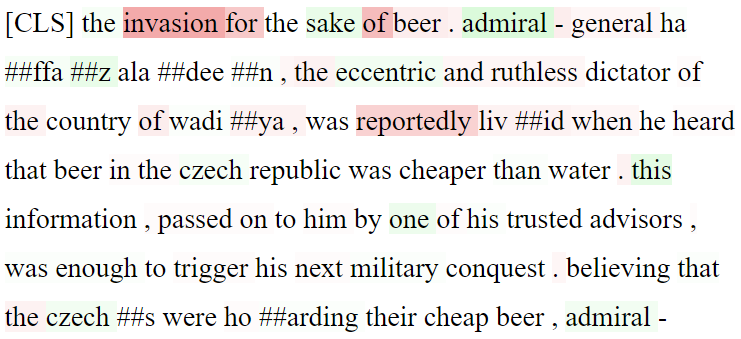
\includegraphics[width=\linewidth]{obrazky-figures/dictator.png}
      \caption{BERT model, correctly classified}
      \label{fig:apend1_a}
    \end{subfigure}%
    \begin{subfigure}{.5\textwidth}
      \centering
      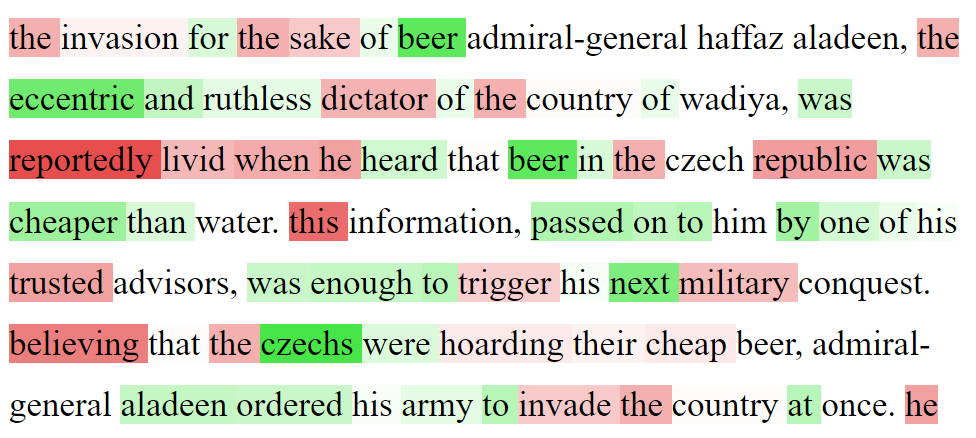
\includegraphics[width=\linewidth]{obrazky-figures/bayes_dictator.png}
      \caption{Baseline model, correctly classified}
      \label{fig:apend1_b}
    \end{subfigure}
    \caption{Interpretability of an unreliable article with the topic of war generated by ChatGPT.}
    \label{fig:apend1}
\end{figure}

Figure \ref{fig:apend1_b} shows an article about North Korea firing ballistic missiles into the sea from a reliable source. Figure \ref{fig:apend2_b} is an unreliable article stating that the covid vaccine is dangerous.


\begin{figure}[H]
    \centering
    \begin{subfigure}{.5\textwidth}
      \centering
      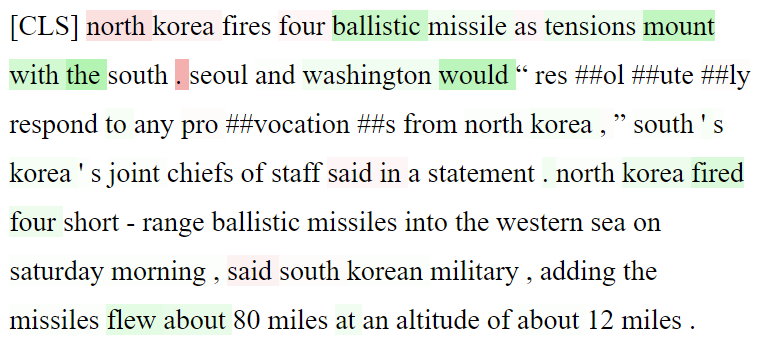
\includegraphics[width=\linewidth]{obrazky-figures/korea_weird.png}
      \caption{Label: reliable, topic: war \\result: correctly classified}
      \label{fig:apend2_a}
    \end{subfigure}%
    \begin{subfigure}{.5\textwidth}
      \centering
      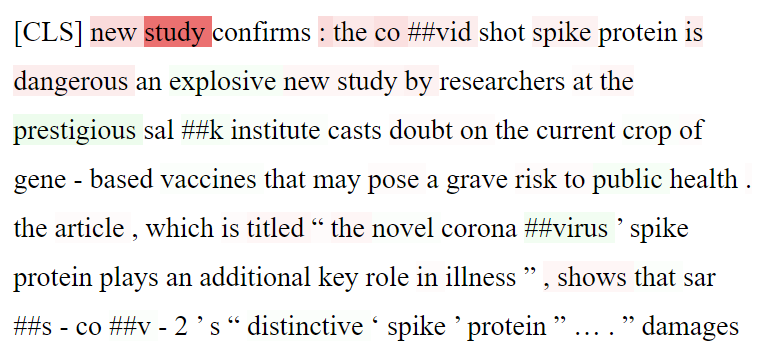
\includegraphics[width=\linewidth]{obrazky-figures/covid2.png}
      \caption{Label: unreliable, topic: covid \\result: correctly classified}
      \label{fig:apend2_b}
    \end{subfigure}
    \caption{Interpretability for two articles by the BERT model.}
    \label{fig:apend2}
\end{figure}


\chapter{Contents of the Enclosed SD card}
The SD card enclosed as part of this thesis consists of the following tree structure: \\

\dirtree{%
    .1 /.
    .2 data \quad \ldots{} \begin{minipage}[t]{10cm}
                        Directory containing all datasets \\
                \end{minipage}.
    .2 src \quad \ldots{} \begin{minipage}[t]{10cm}
                        Directory containing all models and source files \\
                \end{minipage}.
    .3 tutorial.ipynb \ldots{} \begin{minipage}[t]{10cm}
                        This file contains a tutorial showing how to use the created models \\
                \end{minipage}.
    .2 src\_doc \ldots{} \begin{minipage}[t]{10cm}
                        Directory containing all source files of the latex documentation \\
                \end{minipage}.
    .2 doc \quad \ldots{} \begin{minipage}[t]{10cm}
                        Directory containing this pdf file \\
                \end{minipage}.
    .3 thesis{.}pdf \\.
    .2 requirements{.}txt \ldots{} \begin{minipage}[t]{10cm}
                        File containing all required libraries
                \end{minipage}.
}
